\section{Design of FXLMS system} \label{sec:systemDesign}
This appendix will go through the design of the system using a feedforward topology. The ANC system will be placed in a headphone with the microphones placed as seen on \autoref{fig:SystemHeadphone}. A B\&K TYPE 4128-C will be used as the HATS during tests. This means that the cancellation path will have a time invariant impulse response. 


\begin{figure}[H]
	\centering
	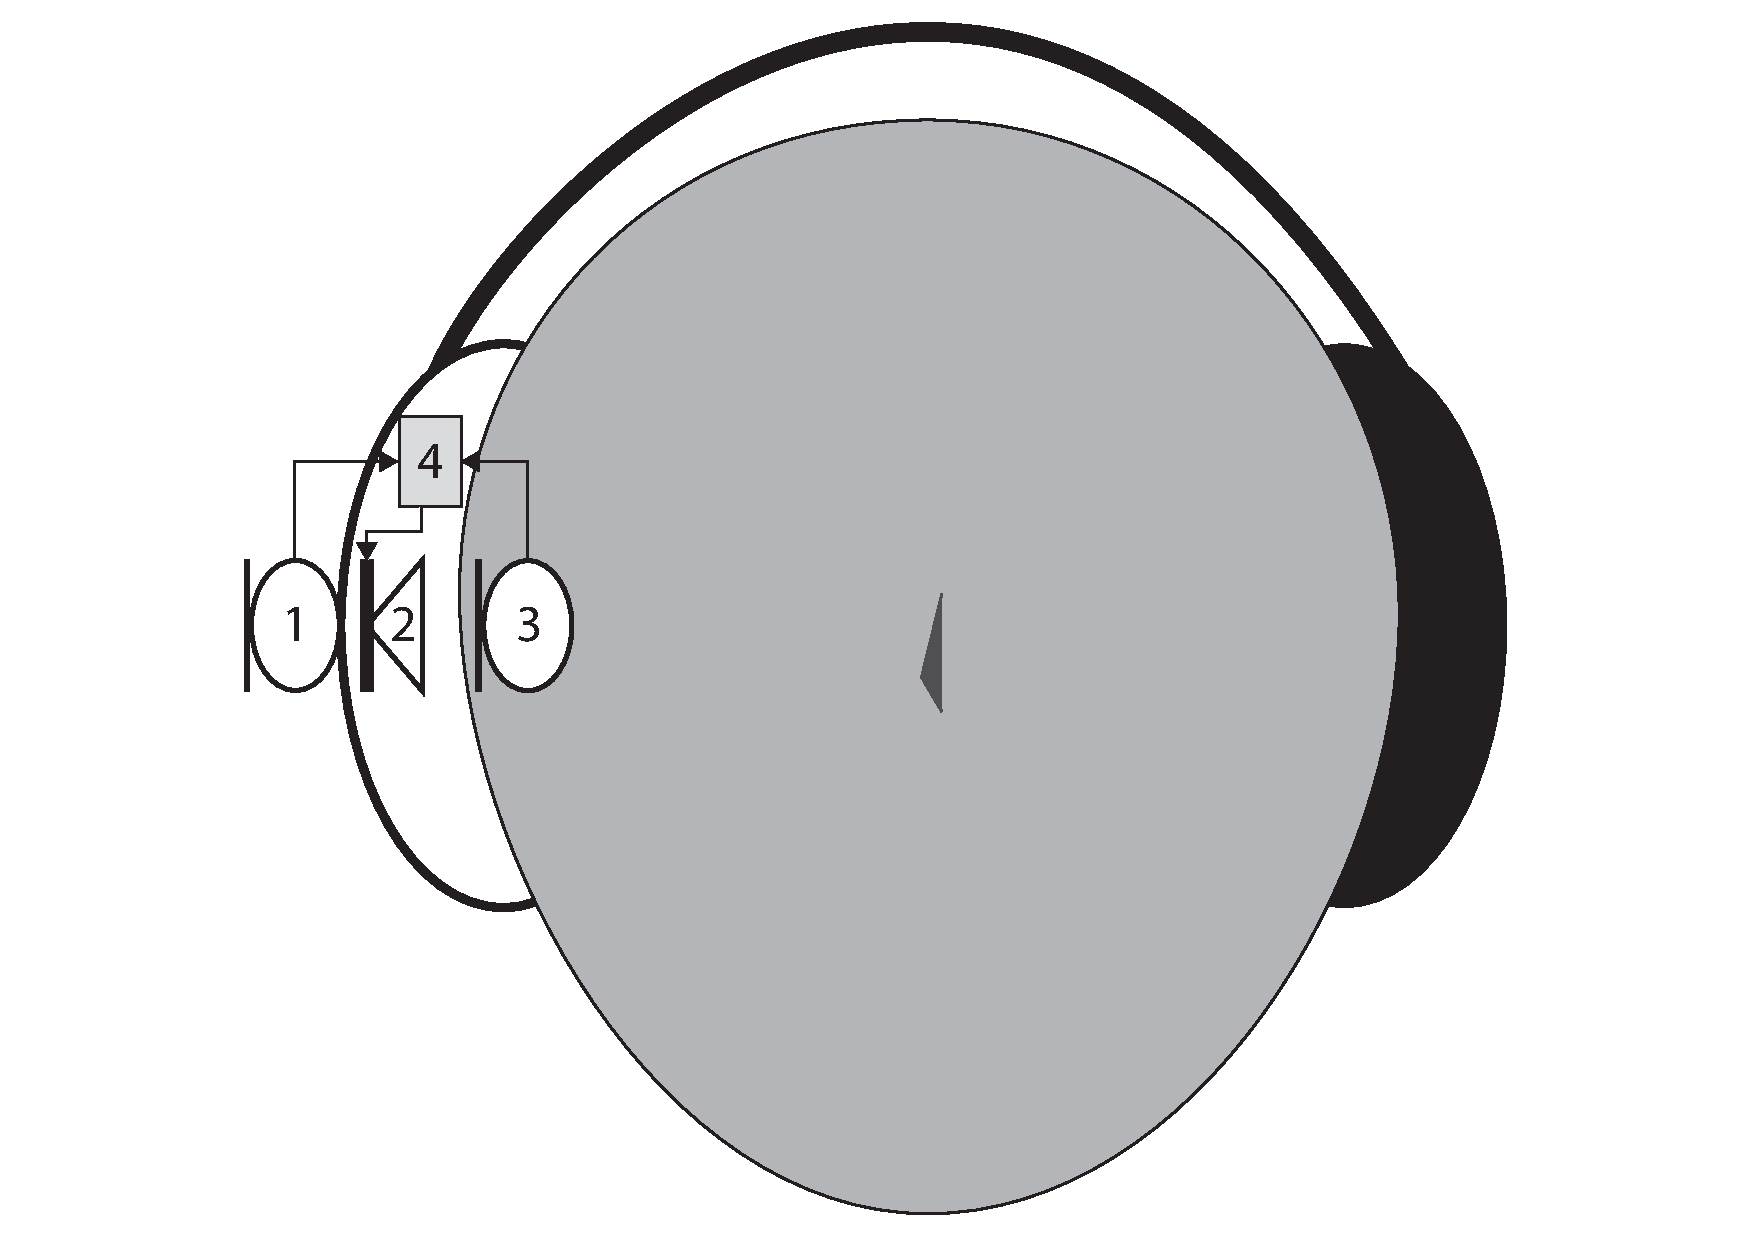
\includegraphics[width=0.8\textwidth]{Articleillustrations/SystemOverview}
	\caption{Illustration of the HATS wearing a headphone fitted with a ANC solution.}
	\label{fig:SystemHeadphone}
\end{figure}  

Because the cancellation path is constant, the adaptive algorithm adjusting the cancellation path (CP) estimate will not be in the basic system. This means that the copy of the CP estimate will be a constant impulse response. The CP has been found as described in \autoref{sec:CPjournal}. The basic feedforward control system is shown in \autoref{fig:BasicSystem}. 

\begin{figure}[H]
	\centering
	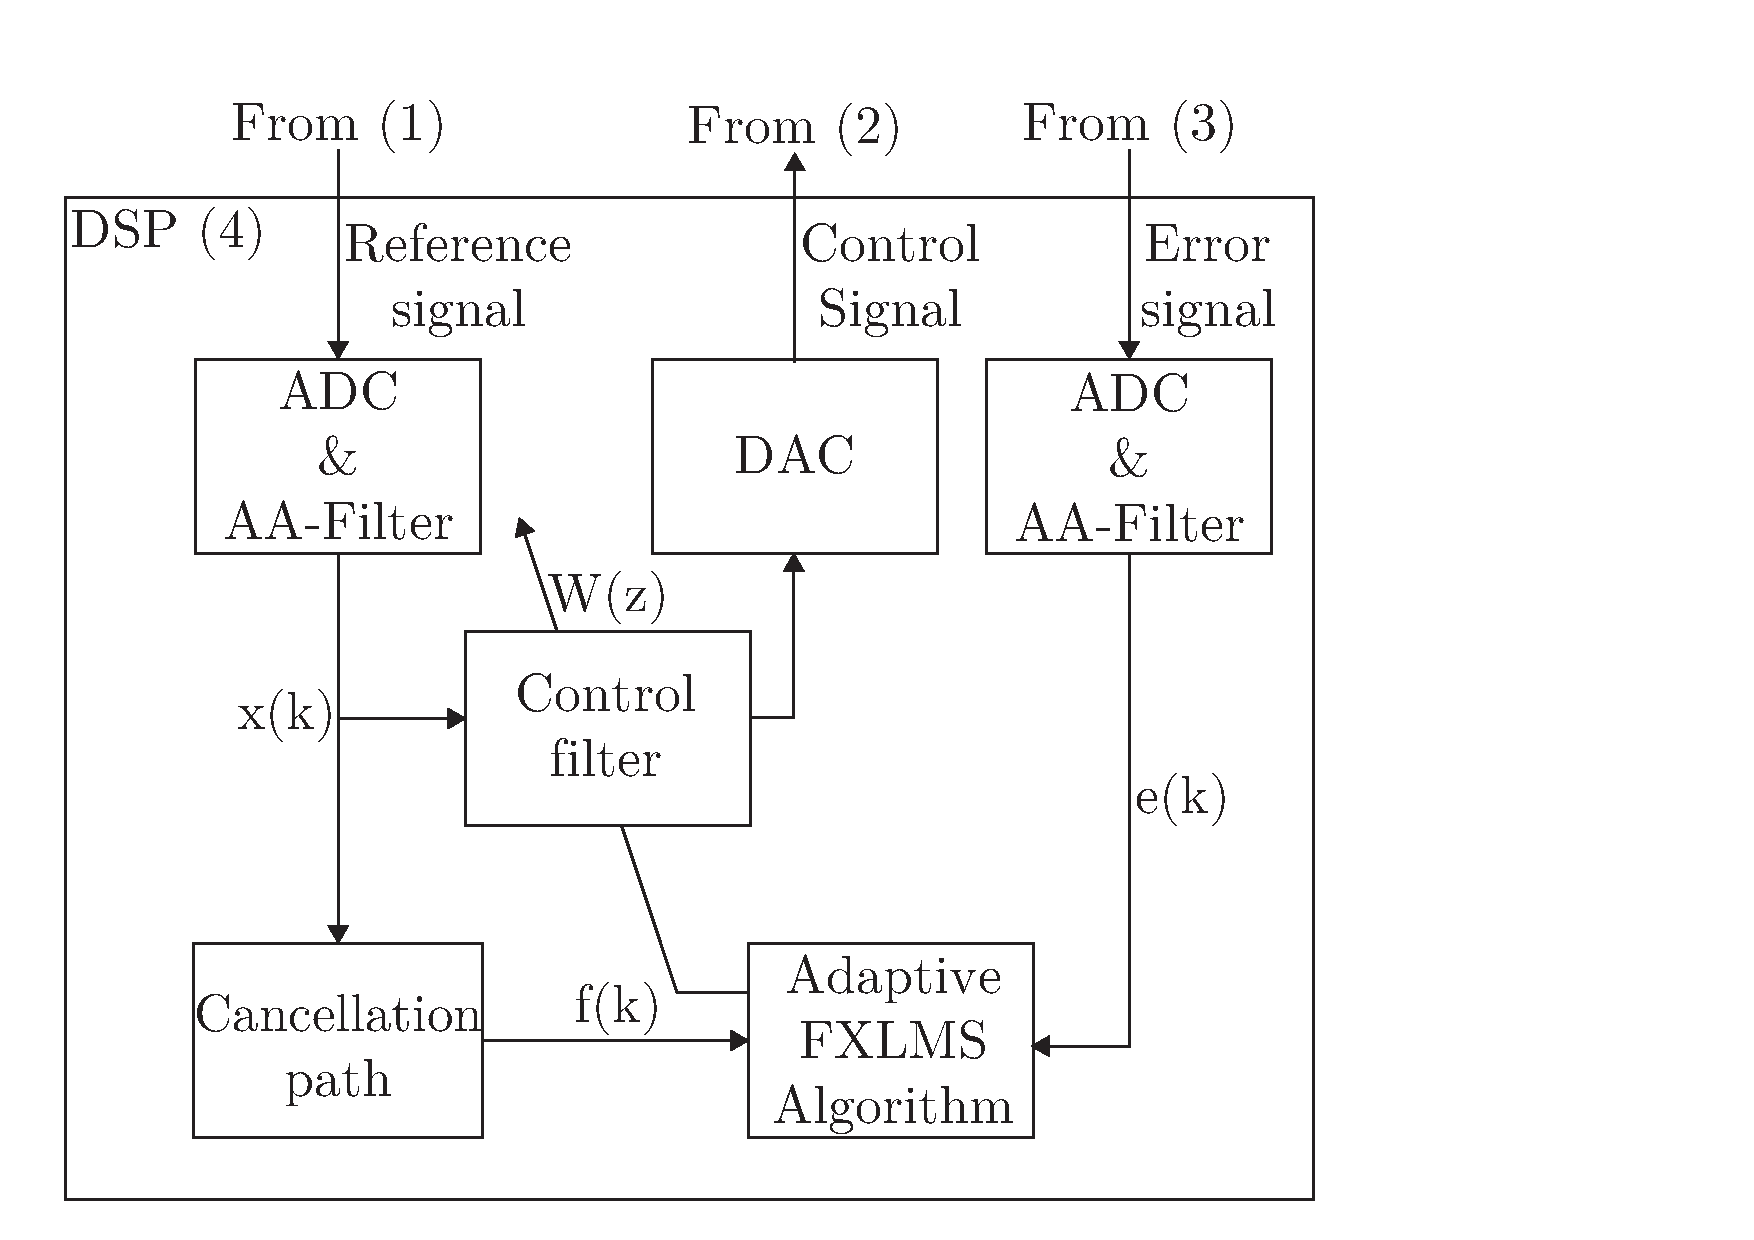
\includegraphics[width=0.75\textwidth]{ArticleIllustrations/ANCFeedForward}
	\caption{Block diagram of basic system without adaptive CP.}
	\label{fig:BasicSystem}
\end{figure}   

\fxnote{Possibly missing text}



\subsection{FXLMS algorithm for FIR filters}\label{subsec:fxlms}
The FXLMS is a gradient descent algorithm which iteratively changes the coefficients of the control filter by adding a calculated step to the current coefficients which should converge to a global minimum of the error criterion. The derivation of the FXLMS algorithm is given below. 
\begin{equation}\label{eq:FXLMSNewCoef}
w(k+1) = w(k) - \mu\nabla J(k)
\end{equation}
Where:
\begin{description}
	\item[\text{$\nabla$J}] is the gradient of the error surface at the location given by the current weight coefficient.
	\item[\text{$\mu$}] is a convergence factor.
	\item[w(k)] is the weight coefficients of the control filter written as  $w(k)=[w_0(k),w_1(k) ,\cdots, w_{L-1}(k)]^T$.
\end{description}
The error is defined as:
\begin{equation}\label{eq:FXLMSError}
e(k) = p(k) + s(k)
\end{equation}
Where:
\begin{description}
	\item[\text{$p(k)$}] is the primary noise source.
	\item[\text{$s(k)$}] is the control source.
\end{description}

The error criterion as a function of the filter weights is to be minimized, therefore the gradient of the error surface ($\nabla J$) is calculated by differentiating the mean squared error (MSE), as shown in equation \ref{eq:FXLMSGradient}.
\begin{equation}\label{eq:FXLMSGradient}
J(k) = e^2(k)
\end{equation}

Differentiating equation \ref{eq:FXLMSGradient} with respect to $w(k)$ yields equation \ref{eq:FXLMSGradientW(k)}. The last substitution can be made because $p(k)$ does not depend on $w(k)$. So the term $p(k)$ from equation \ref{eq:FXLMSError} does not influence the gradient of $e(k)$:

\begin{equation}\label{eq:FXLMSGradientW(k)}
\Delta w(k) = \frac{\partial e^2(k)}{\partial w(k)} = 2e(k)\frac{\partial e(k)}{\partial w(k)} = 2e(k)\frac{\partial s(k)}{\partial w(k)}
\end{equation}
$e(k)$ can be sampled. How to obtain s(k) is described below. \\
The controller output signal y(k) is given by equation \ref{eq:FXLMSOutput}.

\begin{equation}\label{eq:FXLMSOutput}
y(k) = w^T(k) + x(k) = \sum_{i=0}^{L-1} w_i(k)x(k-i)
\end{equation}
Where:
\begin{description}
	\item[x(k)] = $[x(k) x(k-1) \cdots x(k-L+1)]^T $
\end{description}
$s(k)$ can be formulated as equation \ref{eq:FXLMSs(k)}.

\begin{equation}\label{eq:FXLMSs(k)}
s(k) = [w^T(k)x(k)]*c(k)\approx y(k)*\hat{c}(k) = \sum_{i=0}^{M-1}\hat{c}_i(k)y(k-1)
\end{equation}
Where:
\begin{description}
	\item[y(k)] = $[ y(k), y(k-1), \cdots, y(k-M+1)]$
	\item[c(k)] is the impulse response of the cancellation path (filter taps)
\end{description}

Equation \ref{eq:FXLMSs(k)} can be rewritten to equation \ref{eq:FXLMSs(k)2}.

\begin{equation}\label{eq:FXLMSs(k)2}
s(k) = [w^T(k)x(k)]*c(k)\approx w^T(k)*f(k)
\end{equation}
Where:
\begin{description}
	\item[f(k)] is the filtered reference signal $f(k)=x(k)c(k)$
	\item[f(k-j)] = $\sum_{i=0}^{M-1}\hat{c}_i(k)x(k-i-j)$
\end{description}

By using equation \ref{eq:FXLMSs(k)2} substituted into equation \ref{eq:FXLMSGradientW(k)}, the error of the surface gradient can be written as equation \ref{eq:FXLMSNablaJ}:

\begin{equation}\label{eq:FXLMSNablaJ}
\nabla J = 2e(k)\frac{\partial s(k)}{\partial w(k)} = 2e(k)f(k)
\end{equation}

Which yields equation \ref{eq:FXLMSw(k+1)}:

\begin{equation}\label{eq:FXLMSw(k+1)}
w(k+1) = w(k) - 2\mu e(k)f(k)
\end{equation}

Which is the standard FXLMS algorithm when using an adaptive FIR filter.
\begin{equation}\label{eq:FXLMSw_j(k+1)}
w_j(k+1) = w_j(k) - 2\mu e(k)f(k-j)
\end{equation}

With the definition of the FXLMS given, the basic system in \autoref{fig:BasicSystem}, can be simulated.



\subsection{Simulation} 
The basic system shown in \autoref{fig:BasicSystem} has been setup in Simulink\textsuperscript{\textregistered}, as shown in \autoref{fig:SimulinkRealWorld} and \autoref{fig:SimulinkANC} showing the "real world"-simulation and the alogrithm-simulation, respectively.

\begin{figure}[H]
	\centering
	\includegraphics[width=1\textwidth]{figures/BasicSystem/SimulinkRealWorld}
	\caption{Simulink of "real world".}
	\label{fig:SimulinkRealWorld}
\end{figure}    

\begin{figure}[H]
	\centering
	\includegraphics[width=1\textwidth]{figures/BasicSystem/SimulinkANC}
	\caption{Simulink of "ANC algorithm".}
	\label{fig:SimulinkANC}
\end{figure} 

The functions for the different impulse responses and the control filter is a standard sample-by-sample FIR filter, while the FXLMS algorithm is \autoref{eq:FXLMSw_j(k+1)} implemented with a convergence factor of 0.005. This convergence factor is chosen to by experiment to be as large as possible, without getting an unstable system as described by Hansen \cite{Hansen2}. The delay of the ADC and DAC is set to 0 samples.\fxnote{Which results do we need}

\subsection{Results}

\begin{figure}[H]
	\centering
	\tikzsetnextfilename{DelayRatioAppendix}
	% This file was created by matlab2tikz.
%
%The latest updates can be retrieved from
%  http://www.mathworks.com/matlabcentral/fileexchange/22022-matlab2tikz-matlab2tikz
%where you can also make suggestions and rate matlab2tikz.
%
\definecolor{mycolor1}{rgb}{0.00000,0.44700,0.74100}%
\definecolor{mycolor2}{rgb}{0.85000,0.32500,0.09800}%
%
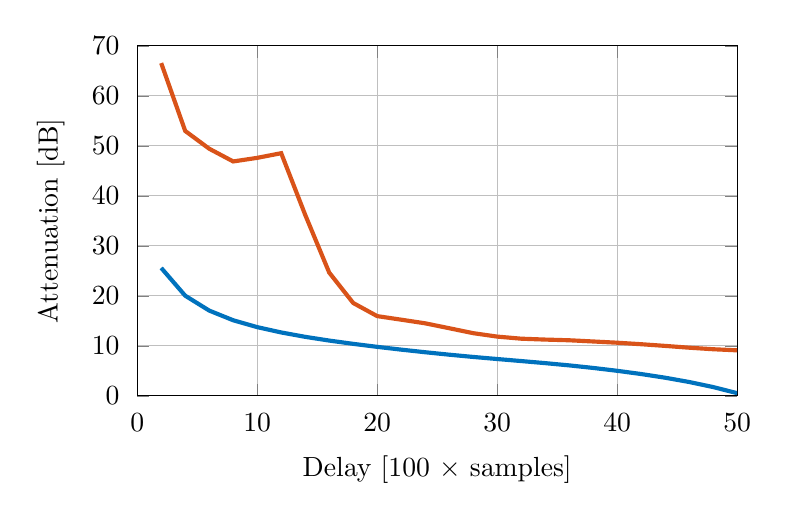
\begin{tikzpicture}

\begin{axis}[%
width=3in,
height=1.75in,
scale only axis,
xmin=0,
xmax=50,
xmajorgrids,
xlabel={Delay [100 $\times$ samples]},
ymin=0,
ymax=70,
ylabel style={yshift=0.3em},
xlabel style={yshift=-0.2em},
ytick={0,10,...,70},
ymajorgrids,
ylabel={Attenuation [dB]},
xticklabel shift={.1cm},
yticklabel shift={.1cm},
axis background/.style={fill=white}
]
\addplot [color=mycolor2,solid,line width=1.5pt,forget plot]
  table[row sep=crcr]{%
2	66.5420250310586\\
4	52.9717264302022\\
6	49.4175149424998\\
8	46.8717703569681\\
10	47.5886347675082\\
12	48.5221420089092\\
14	36.1913078215459\\
16	24.6480360536532\\
18	18.5625963047043\\
20	15.9345988709594\\
22	15.2225924490026\\
24	14.4941735350858\\
26	13.5145912190769\\
28	12.5242379572864\\
30	11.8400523957144\\
32	11.4203165228037\\
34	11.2428861871564\\
36	11.1050592495872\\
38	10.862823901561\\
40	10.6158645117455\\
42	10.3154480278615\\
44	9.97867799972119\\
46	9.61958031033587\\
48	9.31052791122033\\
50	9.08997582022533\\
};
\addplot [color=mycolor1,line width=1.5pt,solid,forget plot]
table[row sep=crcr]{%
	2	25.5751628128288\\
	4	20.0199680852144\\
	6	17.0442763613153\\
	8	15.1060127156582\\
	10	13.7310612019933\\
	12	12.6685774343164\\
	14	11.7903474171974\\
	16	11.0441690144364\\
	18	10.3883064900616\\
	20	9.78797702825996\\
	22	9.23075404560805\\
	24	8.7110676592604\\
	26	8.22176906503967\\
	28	7.77006791263877\\
	30	7.35426684398216\\
	32	6.94907270624338\\
	34	6.5323972441528\\
	36	6.08060777493347\\
	38	5.57101511941803\\
	40	4.99733350616245\\
	42	4.35167702165293\\
	44	3.61433096515684\\
	46	2.757705271237\\
	48	1.74470077738877\\
	50	0.5254168140125\\
};
\end{axis}
\end{tikzpicture}%
	\caption{Attenuation of feedforward FXLMS (blue) compared with feedforward LP FXLMS (red) with different system delays.}
	\label{Fig:delayRatioAppendix}
\end{figure}


